\textbf{COLUNI 2019 -- Questão 32}\par\medskip Leia os textos a seguir:

\par

TEXTO I

O rio que fazia uma volta atrás de nossa casa era a imagem de um vidro mole que fazia uma volta atrás de casa.

Passou um homem depois e disse: Essa volta que o rio faz por trás de sua casa se chama enseada.

Não era mais a imagem de uma cobra de vidro que fazia uma volta atrás de casa.

Era uma enseada.

Acho que o nome empobreceu a imagem.

(BARROS, M. \textbf{Meu quintal é maior que o mundo}. Rio de Janeiro: Objetiva, 2015, p. 85.)

TEXTO II

% COLUNI-AUTO-FIGURES-BEGIN
\begin{figure}[htbp]
\centering
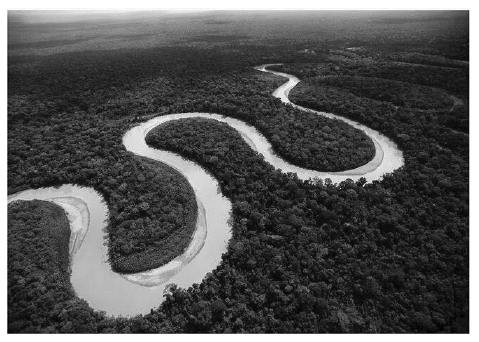
\includegraphics[width=0.95\linewidth]{static/simulados/coluni/figuras/2019/questao-32/figura-1.png}
\end{figure}
% COLUNI-AUTO-FIGURES-END

(Disponível em: <https://br.pinterest.com/pin/758856605931514985/?lp=true>. Acesso em: 3 out. 2018.)

Manuel de Barros retrata a paisagem de um rio de planície com suas voltas e sinuosidade.

O nome das voltas do rio representadas na figura é:
\begin{enumerate}
\item nascentes.
\item afluentes.
\item foz.
\item meandros.
\end{enumerate}
